%-----------------------------------------------------------------
%	PDI DEPENDENCE WITH SST
%	!TEX root = ./../main.tex
%-----------------------------------------------------------------
% \subsection{PDI dependence with SST}\label{sec:pdi-vs-sst}
\subsection{Separation by SST}\label{sec:pdi-vs-sst}
Although in the context of statistics the primary goal of time series analysis is forecasting (as in the ones in figures~\ref{fig:sst-analysis-natl},~\ref{fig:sst-analysis-epac}, and~\ref{fig:global-temps}), we think it's useful to do a time series of the $PDI$ of each basin (figures~\ref{fig:time-series-natl} and~\ref{fig:time-series-epac}) to have more intuitive understanding of the data and to detect any outlying storms we might have missed in~\cref{ssec:dpdi}.

\begin{figure}[H]
	\centering
	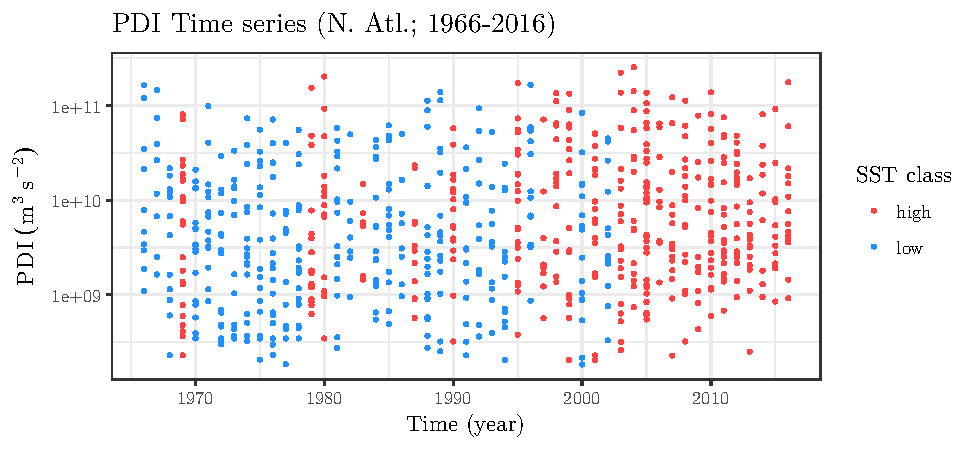
\includegraphics[width=\textwidth]{images/time-series-natl}
	\caption{$PDI$ time series for the Northeast Pacific Ocean}
	\label{fig:time-series-natl}
\end{figure}

\begin{figure}[H]
	\centering
	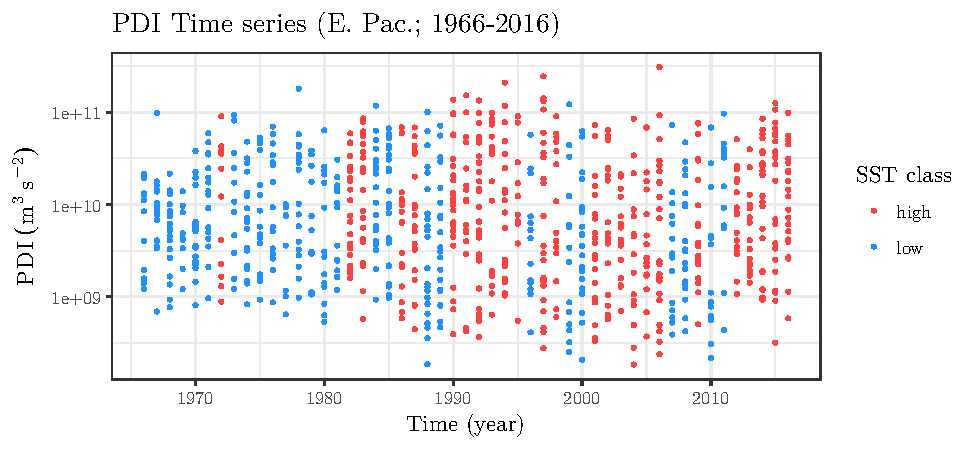
\includegraphics[width=\textwidth]{images/time-series-epac}
	\caption{$PDI$ time series for the Northeast Pacific Ocean}
	\label{fig:time-series-epac}
\end{figure}

As we can see, the data seems quite robust and has no outlying storms (one make an argument about \texttt{CP012006} (2006) in the E.~Pac. being an outlier, but the $PDI$ gap between it and the closest storm by $PDI$ value is quite small when compared to the outliers detected in~\cref{ssec:dpdi}). It's also noticeable the fact that high-SST years have several more storms than low-SST years with a $PDI$ greater than $\SI{e11}{\cubic\m\per\square\s}$, which already seems to confirm the hypothesis brought up in~\cref{ssec:dpdi}. In table~\ref{tab:storms-by-sst-class} we can see a numerical summary of the separation effect on each basin.

\begin{table}[H]
	\centering
	\begin{tabular}{l c c}
		\toprule
		\toprule
		Basin   & $N$ (high-SST) & $N$ (low-SST) \\
		\midrule
		N.~Atl. & \num{406}      & \num{365} \\
		E.~Pac. & \num{599}      & \num{421} \\
		\bottomrule
	\end{tabular}
	\caption{Summary of tropical-cyclones of each basin separated by SST class}
	\label{tab:storms-by-sst-class}
\end{table}

Without further ado, let's examine the $PDI$ density probability distributions presented in figures~\ref{fig:dpdi-by-class-natl} and~\ref{fig:dpdi-by-class-epac}. For these figures we used the \inline{plot_dpdi_by_sst_class()} function defined in the script~\ref{scr:analysis_base}, in~\cref{app:code}), which is nothing more than a slightly tweaked version of the \inline{plot_dpdi()} function.

In essence we see what we predicted in~\cref{ssec:dpdi}: the distribution of high-SST and low-SST years have the same shape, but years with high SST are characterized by tropical-cyclones with larger $PDI$ values. As the $PDI$ integrates the cube of the velocity over the storm life-time, larger $PDI$ values can result from longer lifetimes, larger wind speeds or both. We will try to answer this in the next section.
\begin{figure}[H]
	\centering
	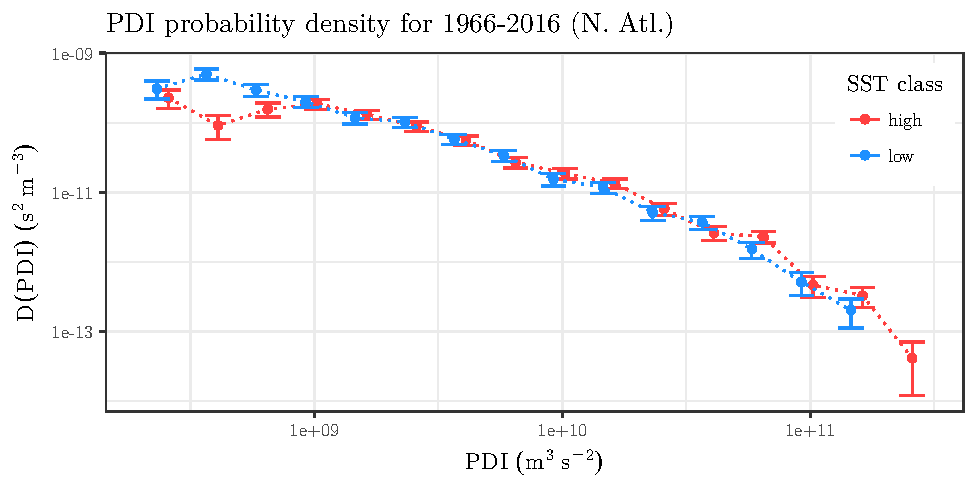
\includegraphics[width=\textwidth]{images/dpdi-by-class-natl}
	\caption{$D(PDI)$ distributions calculated separately for years with high or low SST for the North Atlantic Ocean}
	\label{fig:dpdi-by-class-natl}
\end{figure}

\begin{figure}[H]
	\centering
	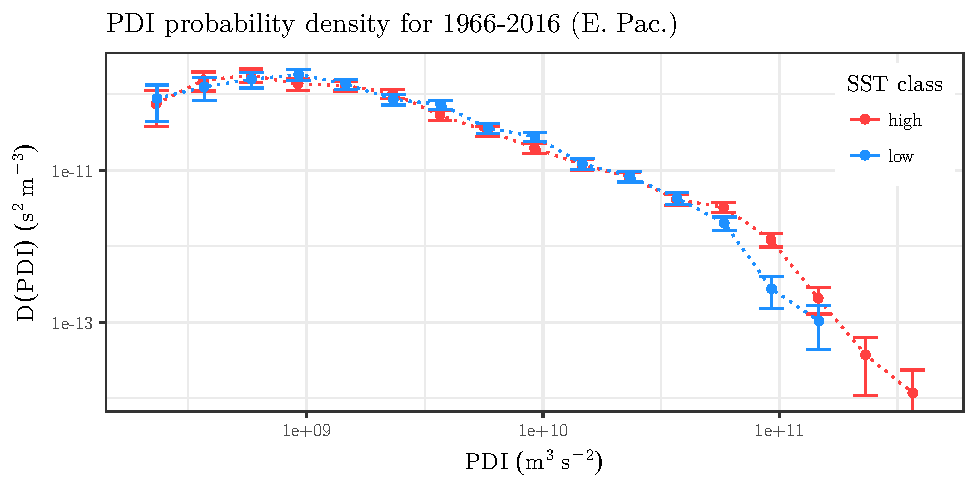
\includegraphics[width=\textwidth]{images/dpdi-by-class-epac}
	\caption{$D(PDI)$ distributions calculated separately for years with high or low SST for the Northeast Pacific Ocean}
	\label{fig:dpdi-by-class-epac}
\end{figure}


